\title{Ciência do solo sem fronteiras}
\author{por Yuri A. Gelsleichter}
\maketitle

\begin{wrapfigure}{l}{0.15\textwidth}
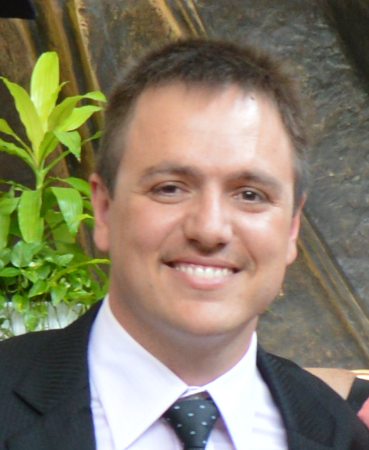
\includegraphics[width=0.15\textwidth]{figuras/yuri-foto}
\end{wrapfigure}

Olá amigo leitor, sou estudante de Engenharia Ambiental e Sanitária da Universidade do Sul de Santa Catarina (\href{http://www.unisul.br/wps/portal/home/}{UNISUL}), intercambista na Hungria, e gostaria de compartilhar com você um pouco de minha experiência no programa Ciência sem Fronteiras (\href{http://www.cienciasemfronteiras.gov.br/web/csf}{CsF}).

Essa história começou no meu ensino médio, após receber em minha turma um aluno vindo da Nova Zelândia. Desde então, tive o interesse de fazer intercâmbio, porém, sempre foi um sonho distante por diversos fatores: dinheiro, família, trabalho, namorada, comodidade, enfim, muitas coisas me prendiam, não sabia se em algum dia, poderia realizar isso, pensei até em morar no estrangeiro por conta própria com intuito do domínio de um segundo idioma e algumas aventuras. Mais recentemente imaginava que talvez o sonho fosse ser realizado através de um programa de mestrado ou doutorado no exterior.

Um dia no caminho para universidade escutando \href{http://conteudo.ebcservicos.com.br/programas/a-voz-do-brasil}{A Voz do Brasil}, ouvi o anúncio que seria lançado o programa de bolsas de estudo no exterior, financiado pelo governo federal. Desde o primeiro edital de CsF em 2011 comecei a me inscrever. Como muitos brasileiros tive a barreira do inglês, mas em nenhuma desisti, fui atrás fiz cursos e provas de inglês. E somente na quarta tentativa de participar do programa, a um semestre de me graduar, consegui a grandiosa oportunidade de fazer intercâmbio na modalidade de graduação sanduíche. Hungria foi meu destino. Largamos toda estabilidade adquirida, eu e minha devota esposa, e partimos sem olhar para trás.\\
\\
\begin{figure}[htbp]
   \centering
   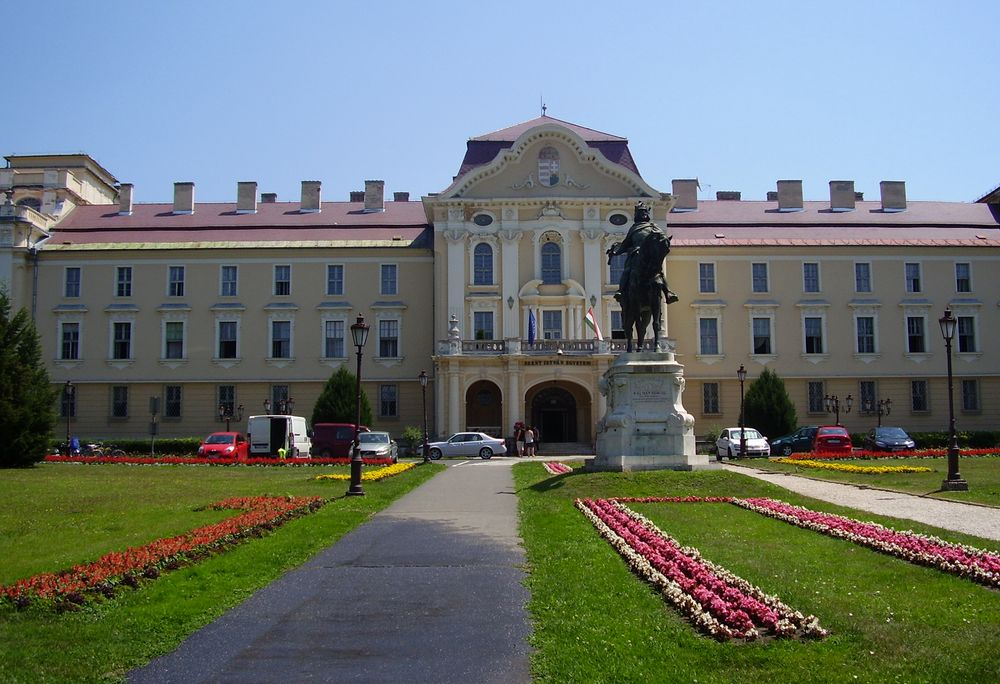
\includegraphics[scale=0.8]{figuras/yuri-foto-5}
   \caption{Prédio principal da Universidade Szent István. Fonte: \href{http://en.wikipedia.org/wiki/G\%C3\%B6d\%C3\%B6ll\%C5\%91}{Wikipédia}.}
   \label{fig:rótulo-da-figura}
\end{figure}
   
Tinha apenas um inglês básico e fui para o curso de dois meses, oferecido pelo programa na Hungria. Chegando ao destino em \href{http://en.wikipedia.org/wiki/G\%C3\%B6d\%C3\%B6ll\%C5\%91}{Gödöllő} na \href{http://sziu.hu/}{Universidade Szent István}, tudo era muito novo a cultura, o idioma, as pessoas, e me perguntava: como serão essas aulas em inglês, será que vou consegui acompanhar? Muitas dúvidas surgiram, mas após o curso intensivo e mais alguns dias de aula senti-me seguro e pronto.

\subsection{Ciência do solo sem fronteiras na Hungria}

No Brasil não tinha uma relação muito próxima dos estudos dos solos, mas gostei de estudar geologia e pedogênese. Na Hungria foram-me ofertadas disciplinas relacionadas ao estudo e conservação dos solos dentre outras. Logo nas primeiras aulas de solos com a professora \href{https://www.linkedin.com/profile/view?id=40499203&authType=NAME_SEARCH&authToken=tTwr&locale=en_US&srchid=1909093141405346286275&srchindex=1&srchtotal=1&trk=vsrp_people_res_name&trkInfo=VSRPsearchId\%3A1909093141405346286275\%2CVSRPtargetId\%3A40499203\%2CVSRPcmpt\%3Aprimary}{Dr. Michelí Erika} e sua equipe muito experientes, desde então tive grande interesse nos estudos dos solos. Intensivamente aprendi o funcionamento do sistema internacional de classificação de solos World Reference Base for Soil Resources (\href{http://www.fao.org/soils-portal/soil-survey/soil-classification/world-reference-base/en/}{WRB}), e paralelamente fui adentrando ao estudo das ciências dos solos e seus processos e características.\\
\\
\begin{figure}[htbp]
   \centering
   \includegraphics[scale=0.8]{figuras/yuri-foto-2}
   \caption{Saída de campo do semestre atual na disciplina \textit{Soil Degradation and Conservation}, envolvendo análise de solo e alteração geológica. Fonte: Arquivo pessoal.}
   \label{fig:rótulo-da-figura}
\end{figure}

Durante as disciplinas cursadas na Szent István tivemos muitas saídas de campo as quais possibilitaram um conhecimento mais direto e palpável, relacionadas principalmente, com o entendimento dos solos.

\subsection{Minha contribuicão ao Brasil}

No edital ao qual estou inserido foi previsto um estágio de trabalho e ou pesquisa. Não era tarefa fácil para a universidade alocar todos os alunos em atividades. Assim, estava aberto para os alunos escolherem suas atividades. Durante as aulas de solos foi utilizado como guia de estudo o WRB 2006. Ao ler no capítulo primeiro, que o texto principal está traduzido para 13 idiomas (chinês, francês, alemão, húngaro, italiano, japonês, letão, lituano, polonês, romeno, russo, espanhol e vietnamês), sugeri a tradução para o português, já que WRB é uma ``linguagem'' internacional e comum de solos, adotada oficialmente na Europa, Africa central e oeste, em outros países, como por exemplo: Itália, México, Noruega, Polônia e Vietnã. As atividades de tradução iniciaram-se após o fim do período de avaliações do primeiro semestre.\\
\\
\begin{figure}[htbp]
   \centering
   \includegraphics[scale=0.8]{figuras/yuri-foto-3}
   \caption{Análise de perfil de solo afetado por sal em saída de campo da  disciplina \textit{Soil Degradation and Conservation}. Fonte: Arquivo pessoal.}
\end{figure}

Segundo a Dr. Érika, que coordena o CsF na Szent István, com o programa houve uma grande troca de informações com o Brasil relacionadas aos dados de solos. Posteriormente houve a liberação do banco de dados dos perfis de solos brasileiros pela Embrapa. Durante o segundo semestre, após congresso mundial de solos na Coreia do Sul, fui convidado pela professora Dr. Érika a participar de um projeto para padronização e homogeneização do banco de dados de solos brasileiros, bem como sua ``tradução para o WRB e Soil Taxonomy US. Esse projeto tem a finalidade de dispor os dados para pesquisa a nível mundial, bem como o mapeamento mundial de solos.\\
\\
\begin{figure}[htbp]
   \centering
   \includegraphics[scale=0.8]{figuras/yuri-foto-1}
   \caption{Saída de campo semestre passado na  disciplina \textit{Modern Soil Observation and Conservation Methods}, com análise de perfis de solo em campo agrícola ao lado do campus da universidade. Fonte: Arquivo pessoal.}
\end{figure}

Segundo a Dr. Érika, também poderemos ser peças chaves no próximo congresso mundial de solos que será sediado no Brasil, devido ao fato do domínio da língua Inglesa e da ``linguagem'' internacional de solos, ou seja, dos nomes e termos técnicos na língua inglesa.

Concluindo, digo que em todos os locais que visitei e conheci pude perceber diferenças em relação ao Brasil, positivas e negativas. Penso que todos os estudantes de intercâmbio trazem dentro de si esses pontos positivos e naturalmente isso tende a gerar bons frutos para a sociedade brasileira tanto na academia como na cidadania.

\address{Yuri A. Gelsleichter\\
  Universidade do Sul de Santa Catarina\\
  \email{yuriplanta@gmail.com}}
%%% Local Variables:
%%% mode: latex
%%% TeX-master: 4th-edition.tex
%%% End: